\section{问题提出}
\subsection{问题背景}

神经网络的计算可表示为带有数据依赖的有向无环图（Directed Acyclic Graph，DAG）。图中的算子完成矩阵运算、向量运算或数据搬运，张量连接前后算子并保存中间结果。执行模型推理或训练，既要安排算子的执行顺序，也要组织输入、中间结果和输出的存储与搬运。多核神经网络处理器（Neural Processing Unit，NPU）为此提供并行计算资源：各核具有矩阵、向量和搬运流水线，以及私有的一级缓存（L1）和统一缓冲区（Unified Buffer，UB）；各核访问共享核外主存（DDR）时，共同竞争固定总带宽。

增加核心数可以使互不依赖的计算同时执行，但每个算子仍需等待其输入数据就绪。若依赖链较长，部分核心会等待前驱计算；若多个核心同时读写DDR，单个请求能够获得的带宽又会下降。因此，计算工作量分配均匀并不意味着各核能同时完成任务。子图的执行次序和数据到达时刻，决定了计算流水线能否持续获得可执行的操作。

子图划分把算子组织为可调度单元。把依赖紧密的算子划入同一子图，有利于减少边界搬运和保留数据复用；但过大的子图也可能压缩跨核并行机会，并增加片上容量压力。细分子图提供更多可调度单元，却可能使同一张量被重复读取。已有DAG分组与调度研究讨论了通信与并行性的共同权衡~\cite{A49}；算子级调度研究也展示了分组方式对并行执行机会的影响~\cite{A08}。划分粒度的选择需要同时考察可释放的并行计算与新增的数据传输。

核心映射决定每个子图由哪个核心执行，核内顺序决定同核子图的先后关系。这两项决策还影响张量在片上存储中的存活区间：使用同一张量的算子相邻执行时，可在数据释放之前完成多次使用；无关操作插入其中时，则可能延长驻留并与其他张量竞争容量。容量不足引发的换出与取回又会增加DDR请求，从而把存储安排与执行时序联系起来。共享只读L2进一步提供核间的数据复用机会，其收益取决于后续算子读取时数据是否已经填充、是否仍然驻留，以及当时的读服务负载。

上述因素共同影响总体任务执行时间（Makespan），即从开始执行到全部任务完成的时间。在给定计算图、硬件参数和固定执行规则下，联合确定子图划分、核心映射与核内顺序，并在执行任务组织和存储层级不同的场景中比较结果。研究重点是解释三项决策如何改变计算等待、边界搬运和数据复用，从而形成能够缩短总体任务执行时间的完整方案。

\subsection{问题重述}

给定计算图、硬件配置及固定执行规则，需要为每个非\texttt{COPY\_IN}\slash\allowbreak\texttt{COPY\_OUT}算子指定子图编号，给出各子图的所属核心和每个核心上的子图顺序。子图须完整覆盖待分配算子，由跨子图依赖形成的子图依赖图必须无环，且每个子图在核内顺序中恰好出现一次。评估程序按照场景重建边界搬运、确定核内固定操作顺序和容量不足时的换入换出，再模拟多核心、流水线与共享带宽上的执行；其输出的总体任务执行时间是主要指标，总额外数据搬运量是次要指标。算法须在全部100个测试用例及固定参数下产生可执行方案，并提供可复现的Python脚本。

问题一对应无核间同步机制的场景A。每个子图独立构成一个执行任务（Task，即向单个核心一次下发的调度单元），所有跨子图依赖均通过DDR交接；同核任务切换等待100周期，跨核前驱任务完成后等待1000周期。需要在2～5核配置下建立子图划分与调度模型并生成方案，尽可能缩短总体任务执行时间，同时控制总额外数据搬运量。正文应按原始整图单核基准，给出1～5核的平均加速比折线图；附录须逐用例列出评估得到的总体任务执行时间与总额外数据搬运量，并提供规定格式的程序附件。

问题二对应具有核间同步机制的场景B。同一核心上的全部子图合为一个执行任务，满足容量与依赖条件时，前一子图的数据可在L1或UB中供后一子图使用；跨核依赖仍经\texttt{COPY\_OUT}/\texttt{COPY\_IN}及500周期同步延迟完成。需要在严格满足L1、UB容量约束下，沿用子图划分、核心映射与核内顺序三个决策，为2～5核配置进一步缩短总体任务执行时间并减少额外搬运。正文同样给出1～5核的平均加速比折线图，附录逐用例报告评估周期与总额外数据搬运量，附件给出可复现程序。

问题三在场景B之上加入所有核心共享的只读二级缓存（L2），按先进先出（First-In, First-Out，FIFO）规则管理，容量为1048576~B、带宽为250~B/周期，读服务带宽与DDR独立。需要研究L2容量和带宽对子图划分与调度的影响，建立相应模型并在核数变化时生成合法方案。正文应给出1～5核下无L2与有只读L2两种配置的对比曲线，并以同核数无L2的总体任务执行时间除以有L2的周期，报告只读缓存相对无L2配置的加速比；附录须逐用例列出两种配置的周期、总额外数据搬运量及字节命中率。


\begin{figure}[htbp]\centering
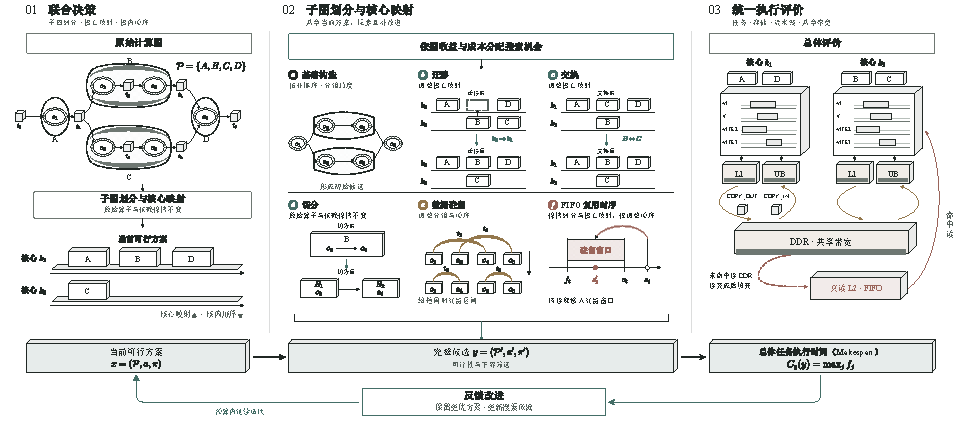
\includegraphics[width=\textwidth]{图片/workflow_qinglu_v7.pdf}
\caption{联合决策、多邻域候选与统一执行评价}\label{fig:roadmap}
\end{figure}

图~\ref{fig:roadmap} 以子图划分 $\mathcal P$、核心映射 $a$ 和核内顺序 $\boldsymbol\pi$ 表示完整方案 $x=(\mathcal P,a,\boldsymbol\pi)$。环节01保存当前可行方案；环节02构造候选；环节03按任务、存储、流水线和带宽约束重建执行过程。评价结果用于保留更优方案，并调整后续候选来源的搜索机会。

环节02展开六种操作：基础构造（a）按拓扑序和分组粒度产生初值；迁移（b）改变一个完整子图的所属核心；交换（c）对调不同核心上的子图；切分（d）将子图分成更细单元，保留原算子及依赖；数据驻留调整（e）通过分组与顺序缩短同时存活的数据区间；FIFO时序调整（f）移动已有子图，使后续读入有机会落入缓存驻留窗口。第一问使用（a）--（d），第二问增加（e），第三问进一步增加（f）。其中（b）--（d）同属结构与负载来源，六种操作围绕同一完整方案交替提出候选。

右侧示意各核心的私有L1、UB与共享DDR。第三问增加只读L2：发射读请求时查询缓存，命中由L2服务，未命中由DDR服务；读完成后按容量条件尝试填充。图中 $f_t$、$e_t$ 是张量 $t$ 的填充和淘汰时刻，$s_t,s'_t$ 是调整前后的读取时刻。新方案会改变这些时刻，故每个候选均通过完整执行评价。评价首先比较总体任务执行时间，周期相同时再比较总额外数据搬运量；搜索结束输出当前方案，第三问再固定该方案进行无L2与有L2配对。
